\newpage
\subsection{Numerical experiment of optimal control problem}
%\subsubsection{Optimal control problem}
\quad In engineering, sometimes we want to know how much heat source provided to receive heat $u(x, t)$ in a physical domain $\Omega$ in a time period $[0, T]$ equals or approximates with $\hat{u}(x, t),\, (x, t)\in Q.$ We suppose that heat source has the form $F(x, t)=f(x, t)+q(x, t)$. This leads to optimize the functional, see \cite{H92-2, H92-3},
\begin{align}\label{J}
	J(q)=\frac{1}{2}\left\|u-\hat{u}\right\|_{L^2(Q)}^2+\frac{\gamma}{2}\left\|q\right\|_{L^2(Q)}^2,
\end{align}
where $q$ being the control variable and $\gamma>0$ being a regularization parameter.

To solve this problem, we use FreeFem++ software which provides an efficient tool called IPOPT. It is designed to perform optimal control problems, for more details see at \cite{A, AL06}. To use this optimizer, we need to include the \textit{ff-Ipopt} dynamic library. The parameters including the objective function $J(f)$ and its gradient $\nabla J(f)$ following
\begin{align}\label{gradJ}
	\nabla J(q)=z(x, t)+\gamma q(x, t),
	\end{align}
	where $z(x, t)$ is the solution of the adjoint problem
	\begin{align}\label{adjoint} 
	\begin{cases}
		-\frac{\partial z(x, t)}{\partial t}+\mathcal{L}z(x, t)=u-\hat{u}, & (x, t)\in Q,\\
		z(x, t)=0, & (x, t)\in S\\
		z(x, T)=0, & x\in \Omega.
	\end{cases}
\end{align}

The gradient $\nabla J(f)$ and adjoint problem will be derived the same as \cite{HTLI14}. Now we will experiment the example as in \cite{DB08}. For the error's sake, we will use Crank-Nicolson method ($\theta=0.5$) to solve the direct problem \eqref{1.1} and adjoint problem \eqref{adjoint}. Consider $\Omega=(0, 1)^2$ and $T=0.1$ and homogeneous Dirichlet boundary condition. The right hand side $f$, the desired state $\hat{u}$ and the initial condition $u_0$ such that
\begin{align*}
	&f(x, t)=-\pi^4w_b(x, T),\\
	&\hat{u}(x, t)=\frac{b^2-5}{2+b}\pi^2 w_b(x, t)+2\pi^2w_b(x, T),\\
	&u_0(x)=\frac{-1}{2+b}\pi^2w_b(x, 0),
\end{align*}
where $w_b(x, t)=e^{b\pi^2 t}\sin(\pi x_1)\sin(\pi x_2), \; b\in \mathbb{R}$.

We chose the regularization parameter $\gamma=\pi^{-4}$ and the optimal solution triple $(\bar{q}, \bar{u}, \bar{z})$ of the optimal control problem \eqref{J} is given by
\begin{align*}
	&\bar{q}(x, t)=-\pi^4\left[w_b(x, t)-w_b(x, T)\right],\\
	&\bar{u}(x, t)=\frac{-1}{2+b}\pi^2w_b(x, t),\\
	&\bar{z}(x, t)=w_b(x, t)-w_b(x, T).
\end{align*}

First, we consider the behavior of the error for a sequence of discretization with decreasing size of the time steps and a fixed spatial triangulation with $N=1089$ nodes. Second, we examine the behavior of the error under refinement of the spatial triangulation for $M=1024$ time steps. We choose the free parameter $b$ to be $-\sqrt{5}$. Error convergence of different cases are shown in Figures \ref{fig:opt_t} and \ref{fig:opt_x}.

\begin{figure}[h!]
	\centering
	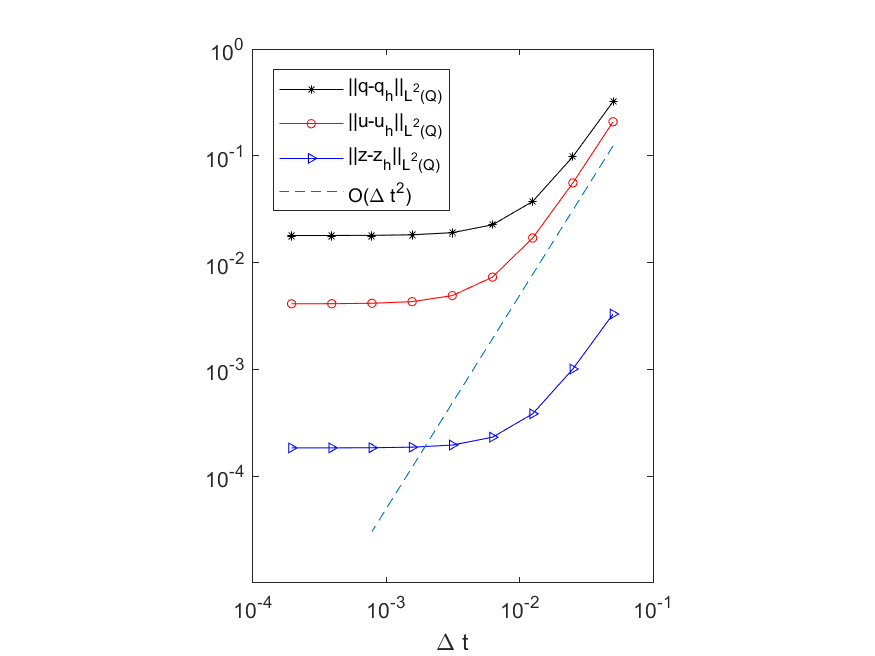
\includegraphics[width=\linewidth]{../freefem++/err_t}
	\caption{Refinement of the time steps for $N =1089$ spatial nodes}
	\label{fig:opt_t}
\end{figure}

\begin{figure}[h!]
	\centering
	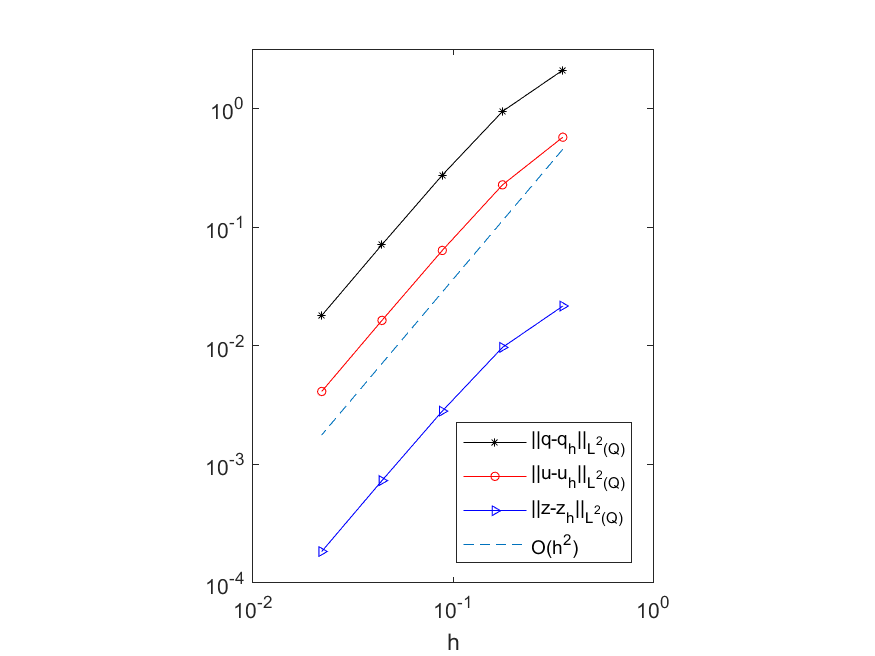
\includegraphics[width=\linewidth]{../freefem++/err_x}
	\caption{Refinement of the spatial triangulation for $M = 1024$ time steps}
	\label{fig:opt_x}
\end{figure}
